\section{Démarche Expérimentale}

\begin{figure}[h]
    \centering
    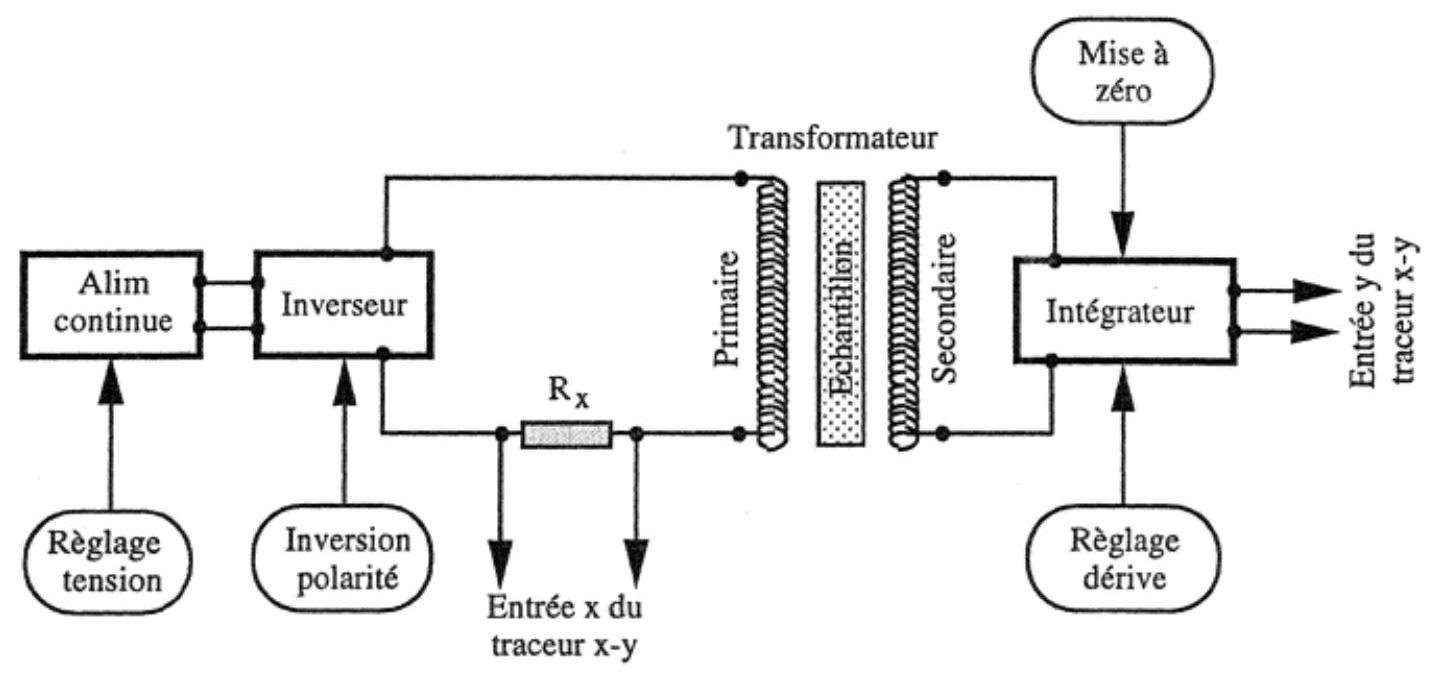
\includegraphics[width=0.8\linewidth]{figures/montage.png}
    \caption{Schéma du montage expérimental \cite{notice}}
    \label{fig:montage}
\end{figure}

Afin de déterminer la perméabilité magnétique de différents matériaux, le montage à la \autoref{fig:montage} est utilisé. Deux transformateurs différents sont utilisés.

\begin{enumerate}
    \item Un transformateur PHYWE, composé d'un noyau en fer en forme de "U" sur lequel il est possible de mettre une bobine primaire et une bobine secondaire. Celles-ci sont modifiables afin de règler la sensibilité du transformateur. Pour cette expérience une bobine primaire de 600 spires et une bobine secondaire de 1200 spires ont été utilisées. Le transformateur peut être fermé avec les échantillons à tester ou avec un bloc PHYWE fourni \cite{bloc_phywe}.
    \item Un transformateur cylindrique, composé d'une bobine primaire de 405 spires et d'une bobine secondaire de 4920 spires. Les échantillons cylindriques à étudier sont inserés à l'intérieur du cylindre.
\end{enumerate}

Avant le début des mesures il est nécessaire de s'assurer que l'intégrateur ne dérive pas entre chaque mesure en réglant son potientomètre pour supprimer le "drift". Pour chaque échantillon, les mesures se font sur un cycle de tension \(0 \rightarrow V_+ \rightarrow V_- \rightarrow V_+\). Les valeurs \((V_i, V_f)\) sont relevées automatiquement par le traceur X-Y, où \(V_i\) est la tension d'entrée mesurée aux bornes d'une resistance \((1.00 \pm 0.01)\) \si{\ohm} à l'entrée du transformateur et \(V_f\) est l'intégrale de la tension de sortie amplifiée du transformateur.